\chapter{Inputs to the Functional Safety Concept}
\label{ch:inputs}

\section{Safety goals from the Hazard Analysis and Risk Assessment}

% Instructions:

% REQUIRED:
% Provide the lane departure warning and lane keeping assistance safety goals as
% discussed in the lessons and derived in the hazard analysis and risk assessment.
 
% OPTIONAL:
% If you expanded the hazard analysis and risk assessment to include other safety goals,
% include them here.

The safety goals for the lane assistance item are presented in Table~\ref{tab:SafetyGoals}

\begin{table}[!htpb]
%\hspace*{-2.0cm}
\caption{Safety Goals}
\begin{center}
\scriptsize
\renewcommand{\arraystretch}{1.4}
\begin{tabular}{ L{3.0cm}|L{9.8cm}  }
 \hline
\rowcolor{black!10}
\textbf{ID} & \textbf{Safety Goal} \\\hline
\textcolor{blue}{\texttt{Safety\_Goal\_01}} &
The oscillating steering torque from the lane departure warning function shall
be limited\\\hline
\textcolor{blue}{\texttt{Safety\_Goal\_02}} &
The lane keeping assistance function shall be time limited and the additional
steering torque shall end after a given time interval so that the driver cannot
misuse the system for autonomous driving.\\\hline
%\textcolor{blue}{\texttt{Safety\_Goal\_03}} & 
%\\\hline
%\textcolor{blue}{\texttt{Safety\_Goal\_04}} &  \\\hline
%\rowcolor{blue!5}
%\texttt{ Measures and Activities} &  \texttt{ Responsibility} & Timeline \\
\end{tabular}
\end{center}
\label{tab:SafetyGoals}
\end{table}

\section{Preliminary Architecture}

% Instructions: 
% Provide a preliminary architecture for the lane assistance item. 
% Hint: See Lesson 3: Item Definition

The preliminary architecture of the lane assistance item is shown in Figure~\ref{fig:pre-arch}.

\begin{figure}[!htpb]
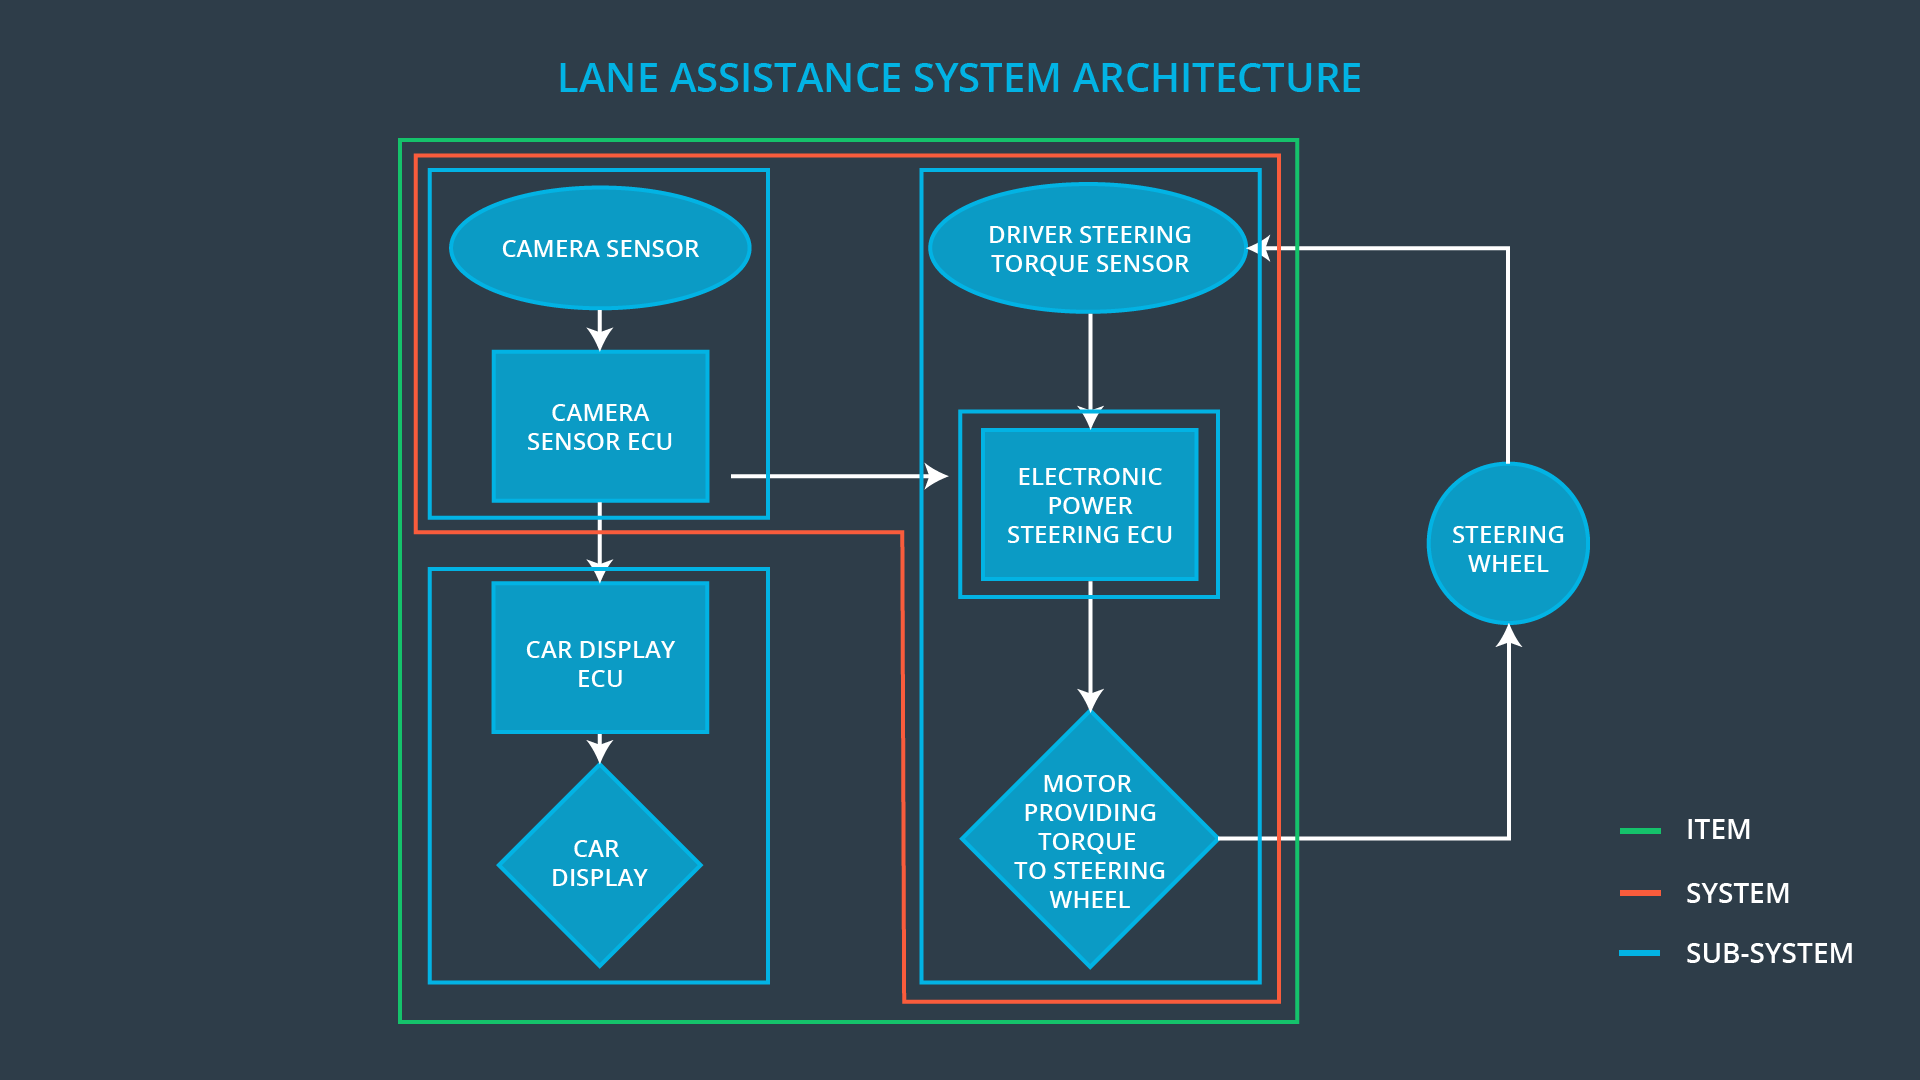
\includegraphics[width=1.00\linewidth]{02-advanced-driver-assistance-system-architecture-01}
\caption{Preliminary architecture}
\label{fig:pre-arch}
\end{figure}


\subsection{Description of architecture elements}

% Instructions: 
% Provide a description for each of the item elements; 
% what is each element's purpose in the lane assistance item?

The functional description of the architecture elements is
shown in Table~\ref{tab:arch-elements}.

\begin{table}[!htpb]
%\hspace*{-2.0cm}
\caption{Architecture elements}
\begin{center}
\scriptsize
\renewcommand{\arraystretch}{1.4}
\begin{tabular}{ L{3.0cm}|L{9.8cm}  }
 \hline
\rowcolor{black!10}
\textbf{Element} & \textbf{Descriptiion} \\\hline
Camera Sensor &
provides Image to the Camera Sensor ECU\\\hline
Camera Sensor ECU &
performs image processing and identifies position of a vehicle w.r.t. the lane\\\hline
Car Display &
displays the status of the lane assistance item\\\hline
Car Display ECU &
accepts packet and displays on a car display if a lane assistance item malfunctions\\\hline
Driver Steering Torque Sensor &
senses the position of the steering wheel\\\hline
Electronic Power Steering ECU &
given current velocity, camera data,  and steering wheel position determines 
whether more input is necessary\\\hline
Motor &
activates vibrations of the steering wheel\\\hline
%\textcolor{blue}{\texttt{Safety\_Goal\_03}} & 
%\\\hline
%\textcolor{blue}{\texttt{Safety\_Goal\_04}} &  \\\hline
%\rowcolor{blue!5}
%\texttt{ Measures and Activities} &  \texttt{ Responsibility} & Timeline \\
\end{tabular}
\end{center}
\label{tab:arch-elements}
\end{table}
